% This is the ADASS_template.tex LaTeX file, 24 Oct 2025.
% It is based on the ASP general author template file, but modified to reflect the specific
% requirements of the ADASS proceedings.

% This is the aspauthor.tex LaTeX file
% Copyright 2021, Astronomical Society of the Pacific Conference Series
% Revision:  29 November 2021

% To compile, at the command line positioned at this folder, type:
% pdflatex ADASS_template
% pdflatex ADASS_template
% This will create a file called ADASS_template.pdf

\documentclass[11pt,twoside]{article}

% Do NOT use ANY packages other than asp2023. 
\usepackage{asp2023}

\aspSuppressVolSlug
\resetcounters

% References must all use BibTeX entries in a .bibfile.
% References must be cited in the text using \citet{} or \citep{}.
% Do not use \cite{}.
% See ManuscriptInstructions.pdf for more details
\bibliographystyle{asp2021}

% The ``markboth'' line sets up the running heads for the paper.
% 1 author: "Surname"
% 2 authors: "Surname1 and Surname2"
% 3 authors: "Surname1, Surname2, and Surname3"
% >3 authors: "Surname1 et al."
% Replace ``Short Title'' with the actual paper title, shortened if necessary.
% Use mixed case type for the shortened title
% Ensure shortened title does not cause an overfull hbox LaTeX error
% See ASPmanual2010.pdf 2.1.4  and ManuscriptInstructions.pdf for more details
\markboth{Zautkin, S.}{BYOM: AI as a Replaceable Part of the Science Platform}

\begin{document}

\title{Bring Your Own Model: Treating AI as a Replaceable Part of the Science Platform}

% Note the position of the comma between the author name and the 
% affiliation number.
% Authors surnames should come after first names or initials, eg John Smith, or J. Smith.
% Author names should be separated by commas.
% The final author should be preceded by "and".
% Affiliations should not be repeated across multiple \affil commands. If several
% authors share an affiliation this should be in a single \affil which can then
% be referenced for several author names. If only one affiliation, no footnotes are needed.
% See ManuscriptInstructions.pdf and ASP's manual2010.pdf 3.1.4 for more details
\author{Serhii Zautkin}
\affil{Canadian Astronomy Data Centre, National Research Council Canada, Penticton, British Columbia, Canada; \email{serhii.zautkin@nrc-cnrc.gc.ca}}

% This section is for ADS Processing.  There must be one line per author. paperauthor has 9 arguments.
\paperauthor{Serhii Zautkin}{serhii.zautkin@nrc-cnrc.gc.ca}{ }{National Research Council Canada}{Canadian Astronomy Data Centre}{City}{British Columbia}{V2A5E3}{Canada}

% There should be one \aindex line (commented out) for each author. These are used to
% build up the author index for the Proceedings. The surname must come first, followed by
% initials. Note the use of ~ before each initial to control spacing.
% The \author entries (see above) have surname last. These \aindex entries have
% surname first.
% The Aindex.py command willl create them for you after you have constructed the \author
% The first entry should be the first author, for bold-facing the author index page-reference

%\aindex{FistAuthor1,~S.~A.}
%\aindex{Author2,~S.~B.}
%\aindex{Author3,~S.}


\begin{abstract}
Two options exist today, and each falls short in a different direction. Point a commercial AI application at data held on a science platform and the science turns into plumbing: credentials, staging, transfers, all for a dataset that should never have moved. Run a coding CLI inside the platform instead and it sits beside the data but sees only a shell and a filesystem — nothing of the archive, the session lifecycle, or the access rules governing them. The first cannot reach the data; the second cannot see the platform. Neither was built for research.
The scientific workbenches now appearing run on the researcher's own machine or cluster so the data need not move. But their domain readiness is built for the life sciences, and the integration path is proprietary: the platform arrives as a plug-in inside the vendor's application, and research context accumulates in that vendor's formats. Astronomy already has platforms tuned over decades to its data models, access rules and standards; we should not have to migrate onto a general-purpose workbench to benefit from these models — the models should meet our platforms on our terms.
I illustrate this with a client over CANFAR, Skaha and the CADC archives whose agent tools are not a parallel API: each performs the same action as a control in the interface, so astronomers and agents share one surface. Both launch, monitor and stop interactive and headless sessions, and the agent can task one with a script in an image carrying the astronomy libraries. Retrieved observations collected in a research area, products land in VOSpace, FITS and cube viewers give a fast visual read the model can be asked to assess, and workflows serve as written protocols the agent follows.
As this work is ongoing, the exact final vision for the user-facing product is still actively taking shape. Rather than presenting a finished system, we present our integration across CANFAR, Skaha, and CADC as the foundation and core of a future AI-enabled science platform. We bring these developments to ADASS to open a dialogue with the community—seeking to learn how researchers envision the natural blend of AI models and research workflows, and how our shared platforms can best deliver that vision.
\end{abstract}

% These lines show examples of subject index entries. At this stage these have to commented
% out, and need to be on separate lines. Eventually, they will be automatically uncommented
% and used to generate entries in the Subject Index at the end of the Proceedings volume.
% Don't leave these in! - replace them with ones relevant to your paper.
%\ssindex{FOOBAR!conference!ADASS 2019}
%\ssindex{FOOBAR!organisations!ASP}

% These lines show examples of ASCL index entries. At this stage these have to commented
% out, and need to be on separate lines. Eventually, they will be automatically uncommented
% and used to generate entries in the ASCL Index at the end of the Proceedings volume.
% The ascl.py command will scan your paper on possible code names.
% Don't leave these in! - replace them with ones relevant to your paper.
%\ooindex{FOOBAR, ascl:1101.010}


\section{AI and Science Platform}
Last year, we presented a StarAI project developed within Herzberg Astronomy and Astrophysics Research Centre R\&D initiative. StarAI was a pathfinder for the place and role of AI within CANFAR platform and Skaha APIs. The architecture and deployment infrastructure of the CANFAR Science Platform is web based and our last year solution was around that vision where we deployed a set of web services (MCP client, MCP server, RAG database etc).

\newpage 
\articlefigure[width=1\textwidth]{web_arch_old.png}{ex_fig1}{StarAI architecture as presented at ADASS XXXV.}
% It is possible to reduce the size of a figure among other changes (see the instructions).  Here is an example:
% \articlefigure[width=.5\textwidth]{example_image}{ex_fig1_reduced}{Welcome to 1953 a little smaller.}


There are a few issues that made this architecture questionable:
\begin{itemize}
\item Who will host an AI model, or who will pay for the API calls to AI model
\item Multiple services running on the CADC infrastructure increasing load on the team and reducing compute resources for research
\item Which AI model to run (cost / efficiency, vendor lock-in etc.)
\item Using Bring Your Own Key model increases security risks, such as breach and theft
\end{itemize}

\section{Multiple Ways to Connect AI}
In the last two years, users have discovered a few ways to integrate artificial intelligence (AI) into their workflows. There are few patterns of connecting AI models:
\begin{itemize}
\item Chat box inside the app (web app or native application) – Gmail webapp
\item Dedicated AI agent inside the app – Slack
\item Command-line interface (CLI)  based application – Claude Code
\item Model-context protocol (MCP) based server connected to the app – Blender
\item Dedicated AI-centred applications – Cursor,  Claude Desktop
\end{itemize}

\section{An AI First Native Architecture}
To address issues from the last year's implementation of AI model integrations with the CADC services and taking into account the availability of desktop applications and CLIs from major AI model vendors, we present a new architecture of connecting Science Platforms to AI models and agentic workflows. 

\articlefigure[width=1\textwidth]{app_arch.png}{ex_fig2}{AI-Ready Science Platform architecture. All product names and logos are trademarks of their respective owners.}

We combined MCP client and server into an operating system native application and moved to user preferred platforms: Windows, macOS, Linux (Omarchy is an Arch based distro, and Ubuntu is Debian based). Secondly, we exposed application supported MCP tools via MCP stdin/stdout bridge (Unix socket underneath), so AI agents can connect to them and invoke procedure calls via JSON-RPC. Finally, we connected the native application with the Science Platform APIs such as Skaha and CANFAR. The application is available in the stores \citep{Zautkin2026Verbinal} today.

There are multiple benefits of such architecture from the development, deployment, and maintenance perspectives as well as from user experience. 

\paragraph{Development benefits}The application development was facilitated by the AI models (Fable 5.1 and Opus 5.5) and the whole process was arranged around translating Skaha and CANFAR APIs into the application functionality and wrapping them into callable MCP tools.

\paragraph{Deployment benefits}
The application does not require any additional hosting services from the CADC but is distributed via relevant platform stores (Apple App Store for macOS version and Microsoft Store for Windows version).

\paragraph{Maintenance benefits}
AI-assisted software development made it possible to address any issues revealed after store approval and application update and user installation.

\paragraph{Personal and User Friendly}
A desktop native application that connects to the Compute and Data resources and keeps research work personal. An AI enabled Science Platform assists users to quickly get around and learn all the complex features that platform has, reducing onboarding time and leveling the learning curve.


\paragraph{Supports Research}
The Science Platform implementation with functionality that helps preserve data and decisions while assisting research workflows.

\paragraph{AI work visibility}
An AI enabled Science Platform visually and audibly informs users about AI agent interactions with the platform.

\paragraph{100\% AI enabled}
Native Science Platform exposes all its functionality as MCP tools that an AI agent understands and can freely communicate with.

\paragraph{AI vendor agnostic}
The MCP bridge is AI model vendor agnostic and works with any of the frontier AI model providers and model routers.

\paragraph{Control AI agents}
MCP bridge and implemented guardrails allow users to set boundaries for AI agents, defining exactly where and how a researcher needs assistance.

\paragraph{Logs and permissions}
Science platform enables logging all agent interactions with application MCP tools, as well as requesting approval for selected actions or destructive actions.
\\
\acknowledgements Built using the Canadian Astronomy Data Centre (CADC) archives and the CANFAR platform.

\bibliography{P105}  % For BibTex

\vspace{1.2em}
\begin{center}
  \begin{minipage}[t]{0.42\textwidth}
    \centering
    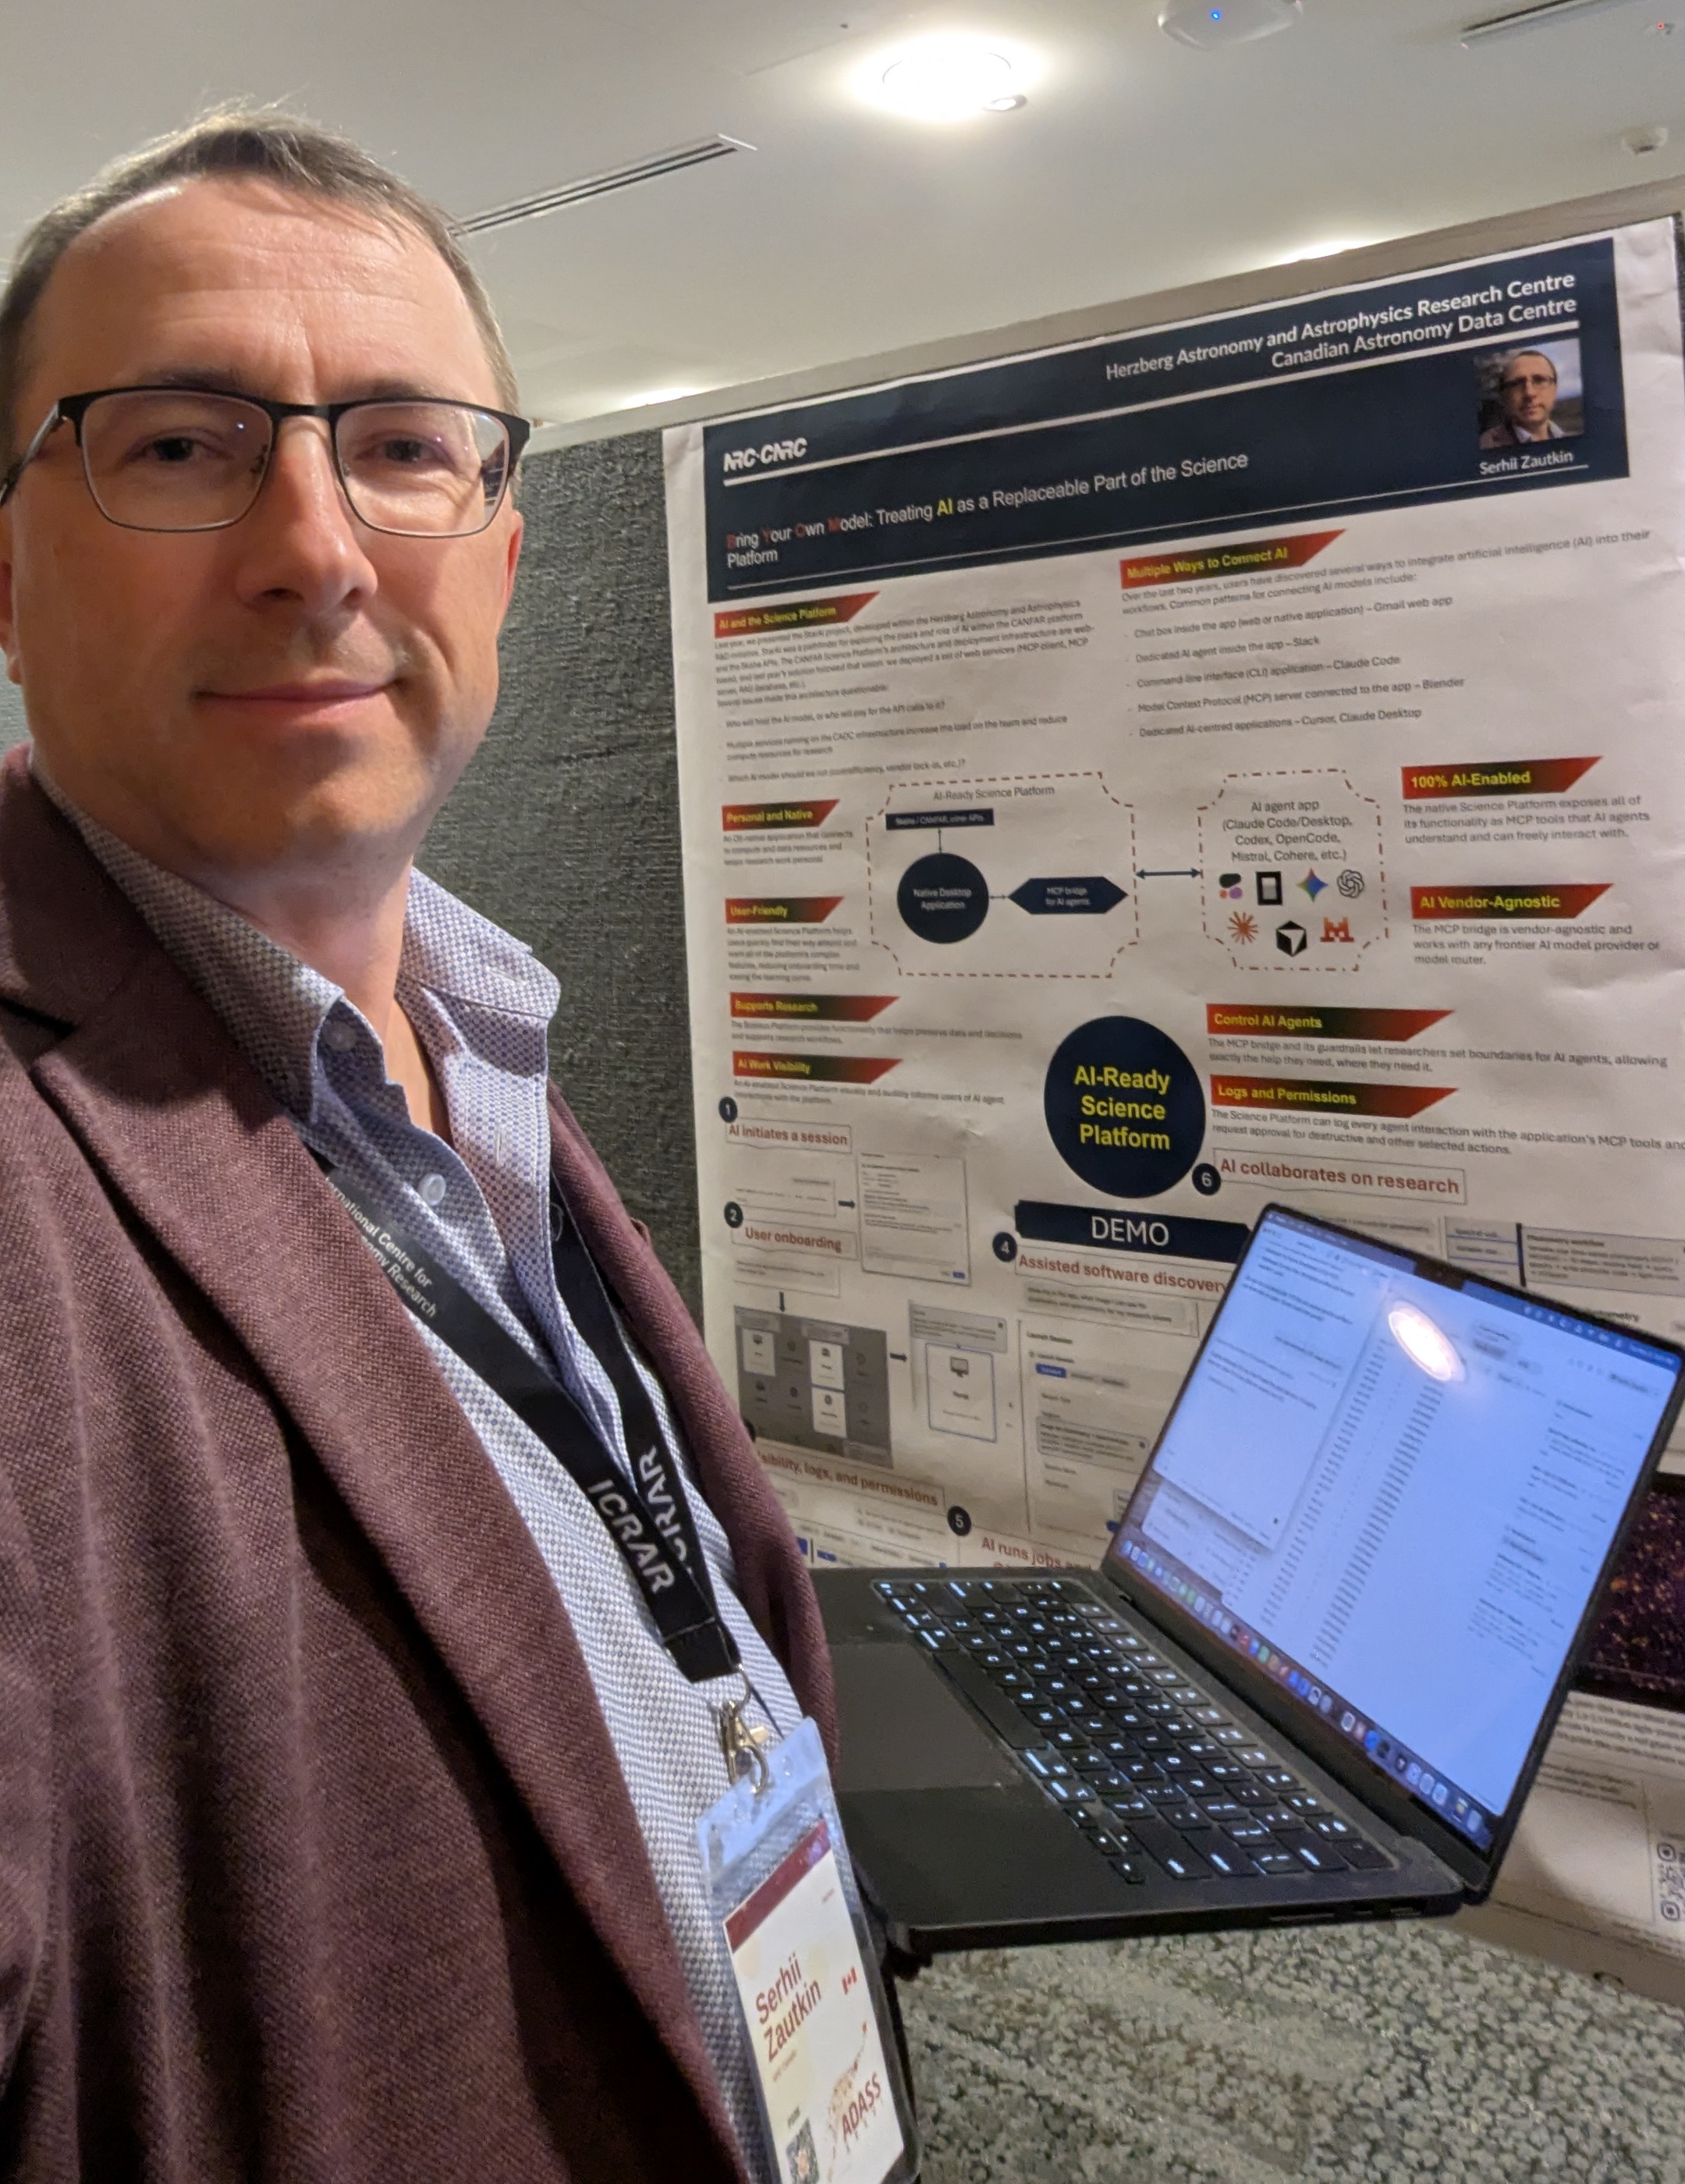
\includegraphics[width=0.55\linewidth]{presenting.jpg} \\[0.4em]
    \small Presenting at ADASS XXXVI. (Photo: Serhii Zautkin)
  \end{minipage}
  \hspace{0.06\textwidth}
  \begin{minipage}[t]{0.42\textwidth}
    \centering
    
\includegraphics[width=0.8\linewidth]{qr_astore.jpg} \\[0.4em]
    \small Apple App Store link
  \end{minipage}
\end{center}
\end{document}
